\chapter{Gelombang Terpandu dan Rongga}\label{ch:b2:guided-waves}

Pulsa sebuah radar berjalan dari pemancarnya ke piringannya di dalam
pipa tembaga bersegi empat; cahaya sebuah sambungan internet berjalan sepuluh
ribu kilometer di dalam benang kaca yang lebih tipis daripada sehelai rambut;
gelombang mikro sebuah oven memantul-mantul di antara dindingnya lalu menetap menjadi
pola bintik panas dan dingin. Sebuah gelombang yang terkurung dinding yang menghantar atau
membiaskan bukan lagi gelombang bidang yang bebas pergi ke mana pun: ia
harus memenuhi syarat batas pada dindingnya, dan itu memilih
bentuk yang boleh diambilnya --- yaitu \emph{ragam}-nya --- dan melarangnya di bawah
frekuensi \emph{ambang}. Bab ini membangun pandu yang paling sederhana, dua
keping penghantar yang sejajar, dari pemantulan
\cref{ch:b2:wave-interfaces}; lalu \omterm{prop:b2:guided-waves:rectangular}{pandu gelombang bersegi empat},
rongga tertutupnya, dan, dalam gambaran sinar, \omterm{prop:b2:guided-waves:fibre}{serat optik}.

\section{Gelombang di antara dua keping penghantar}

\begin{proposition}[Ragam pandu keping sejajar]\label{prop:b2:guided-waves:plates}
\index{pandu gelombang}\index{gelombang terpandu}\index{ragam (pandu gelombang)}\index{frekuensi ambang (pandu gelombang)}
Dua bidang \omterm{prop:b2:wave-interfaces:conductors}{penghantar sempurna} $y = 0$ dan $y = a$ membatasi ruang hampa.
Carilah gelombang yang berjalan sepanjang $z$ dengan $\vect E = E(y)\,\eu^{\iu(\omega t - k_gz)}
\vect e_x$ (medannya sejajar kepingnya, tegak lurus arah
rambatnya). \omterm{thm:b2:maxwell-equations:maxwell}{Persamaan Maxwell} dalam hampa dan syarat $E = 0$
pada kepingnya memaksakan
\[
E(y) = E_0\sin\frac{n\pi y}a , \qquad
k_g^2 = \frac{\omega^2}{c^2} - \Bigl(\frac{n\pi}a\Bigr)^2 , \qquad n = 1, 2, \dots
\]
Ragam $n$ hanya merambat di atas \emph{frekuensi ambang}-nya $f_n = nc/2a$;
di bawahnya, $k_g$ khayal dan medannya meluruh sepanjang pandunya. \omterm{def:b2:dispersion-wave-packets:relation}{Kecepatan
fase} dan grupnya adalah
\[
v_\varphi = \frac c{\sqrt{1 - f_n^2/f^2}} > c , \qquad
v_g = c\sqrt{1 - f_n^2/f^2} < c , \qquad v_\varphi v_g = c^2 ,
\]
dan medan magnetnya mempunyai komponen sepanjang $y$ dan sepanjang $z$: sebuah
\omterm{prop:b2:guided-waves:plates}{gelombang terpandu} tidak transversal dalam arah rambatnya.
\end{proposition}

\begin{proof}
Sisipkanlah ke dalam $\Delta\vect E = \partial_t^2\vect E/c^2$: $E'' - k_g^2E = -(\omega^2/c^2)E$, yakni
$E'' + (\omega^2/c^2 - k_g^2)E = 0$, yang penyelesaiannya yang lenyap di $y = 0$ dan
$y = a$ adalah sinus dengan $\omega^2/c^2 - k_g^2 = (n\pi/a)^2$; $\operatorname{div}
\vect E = 0$ berlaku karena $E_x$ tidak bergantung pada $x$. Faraday memberi
$\underline B_y = (k_g/\omega)\underline E$ dan $\underline B_z = (\iu/\omega)\partial_y\underline E$, yang terakhir
dalam kuadratur. Kecepatannya menyusul dari bentuk Klein--Gordon
\omterm{def:b2:dispersion-wave-packets:relation}{hubungan dispersinya} (\cref{ch:b2:dispersion-wave-packets}).
\end{proof}

\begin{remark}[Ragam sebagai dua gelombang bidang]\label{rem:b2:guided-waves:zigzag}
$\sin(n\pi y/a)\eu^{-\iu k_gz}$ adalah jumlah dua gelombang bidang bervektor
gelombang $(0, \pm n\pi/a, k_g)$, bermodulus $\omega/c$, yang memantul-mantul di antara
kepingnya pada sudut $\theta$ dari sumbunya dengan $\cos\theta = k_gc/\omega$:
sebuah ragam terpandu adalah gelombang bidang yang berjalan zigzag di antara dindingnya, terpantul
dengan $r = -1$ pada masing-masingnya, dan \omterm{prop:b2:waves-on-strings:modes}{gelombang berdiri} transversalnya merupakan
syarat bahwa ia berinterferensi membangun dengan dirinya sendiri. Energinya
berjalan sepanjang zigzagnya dengan $c$, maka sepanjang sumbunya dengan $c\cos\theta = v_g$;
perpotongan puncaknya dengan sumbunya berlari dengan $c/\cos\theta = v_\varphi$. Pada
ambangnya gelombangnya memantul bolak-balik menyeberangi pandunya lalu tak pergi
ke mana pun.
\end{remark}

\begin{omfigure}
\begin{tikzpicture}[font=\small, x=1cm, y=1cm, >=Stealth]
  \begin{scope}
    \draw[thick] (-3,0) -- (3,0); \draw[thick] (-3,2) -- (3,2);
    \fill[pattern=north east lines] (-3,-0.15) rectangle (3,0); \fill[pattern=north east lines] (-3,2) rectangle (3,2.15);
    \draw[omDef, thick, ->] (-2.8,0.2) -- (-1.6,1.8); \draw[omDef, thick, ->] (-1.6,1.8) -- (-0.4,0.2); \draw[omDef, thick, ->] (-0.4,0.2) -- (0.8,1.8); \draw[omDef, thick, ->] (0.8,1.8) -- (2.0,0.2); \draw[omDef, thick, ->] (2.0,0.2) -- (2.8,1.27);
    \draw (-0.4,0.2) -- (0.6,0.2); \draw (0.3,0.2) arc[start angle=0, end angle=53, radius=0.7]; \node[font=\footnotesize] at (0.75,0.55) {$\theta$};
    \draw[->, thick] (-3,-0.6) -- (3,-0.6) node[right, font=\footnotesize] {$z$};
    \node[font=\footnotesize] at (-3.3,1) {$a$};
    \draw[<->] (-3.15,0) -- (-3.15,2);
  \end{scope}
  \begin{scope}[xshift=8.4cm]
    \draw[thick] (0,0) -- (0,2); \draw[thick] (3.6,0) -- (3.6,2);
    \fill[pattern=north east lines] (-0.15,0) rectangle (0,2); \fill[pattern=north east lines] (3.6,0) rectangle (3.75,2);
    \draw[omThm, thick, domain=0:3.6, samples=50] plot (\x,{1+0.8*sin(50*\x)});
    \draw[omProp, thick, domain=0:3.6, samples=50] plot (\x,{1+0.6*sin(100*\x)});
    \draw[dashed] (0,1) -- (3.6,1);
    \node[omThm, font=\footnotesize] at (1.8,2.3) {$n = 1$}; \node[omProp, font=\footnotesize] at (0.9,1.9) {$n = 2$};
    \draw[<->] (0,-0.3) -- (3.6,-0.3) node[midway, below, font=\footnotesize] {$a$ (sumbu $y$)};
  \end{scope}
\end{tikzpicture}

{\small Kiri: sebuah ragam terpandu adalah gelombang bidang yang memantul-mantul di antara
kepingnya; sudut $\theta$ membuka ketika frekuensinya mendekati ambangnya.
Kanan: profil transversal $E(y)$ kedua ragam pertamanya, yang lenyap
pada dinding penghantarnya.}
\end{omfigure}

\begin{omfigure}
\begin{tikzpicture}
\begin{axis}[omaxis, axis x line=bottom, axis y line=left, width=6.6cm, height=4.8cm,
    xlabel={$k_g$}, ylabel={$\omega$}, xmin=0, xmax=3, ymin=0, ymax=4, xtick=\empty, ytick={1,2,3}, yticklabels={$\omega_1$, $\omega_2$, $\omega_3$}, samples=80,
    xlabel style={at={(axis description cs:1.0,0.0)}, anchor=west},
    ylabel style={at={(axis description cs:0.0,1.0)}, anchor=south}]
  \addplot[omThm, thick, domain=0:3] {sqrt(1+x*x)};
  \addplot[omThm, thick, domain=0:3] {sqrt(4+x*x)};
  \addplot[omThm, thick, domain=0:3] {sqrt(9+x*x)};
  \addplot[omDef, dashed, domain=0:3] {x};
  \node[font=\scriptsize, anchor=west] at (axis cs:2.2,2.05) {$\omega = ck_g$};
\end{axis}
\end{tikzpicture}
\hfill
\begin{tikzpicture}
\begin{axis}[omaxis, axis x line=bottom, axis y line=left, width=6.6cm, height=4.8cm,
    xlabel={$f/f_1$}, ylabel={$v/c$}, xmin=1, xmax=4, ymin=0, ymax=2.5, xtick={1,2,3,4}, ytick={1}, samples=100,
    xlabel style={at={(axis description cs:0.5,-0.12)}, anchor=north},
    ylabel style={at={(axis description cs:-0.1,0.5)}, rotate=90, anchor=south},
    legend style={font=\scriptsize, at={(0.97,0.95)}, anchor=north east, draw=none, fill=none}]
  \addplot[omThm, thick, domain=1.05:4] {1/sqrt(1-1/(x*x))};
  \addplot[omDef, thick, domain=1:4] {sqrt(1-1/(x*x))};
  \addplot[black, dashed, domain=1:4] {1};
  \legend{$v_\varphi$, $v_g$}
\end{axis}
\end{tikzpicture}

{\small Kiri: kurva dispersi ketiga ragam pertama sebuah
pandu, masing-masing sebuah hiperbola yang bermula pada ambangnya. Kanan: \omterm{def:b2:dispersion-wave-packets:relation}{kecepatan fase} dan
grup sebuah ragam terhadap frekuensi; energinya merangkak dekat
ambangnya lalu mendekati $c$ jauh di atasnya.}
\end{omfigure}

\begin{example}[Angka]\label{ex:b2:guided-waves:numbers}
Keping yang terpisah \qty{3}{cm}: $f_1 = \qty{5}{GHz}$, $f_2 = \qty{10}{GHz}$; di antara
kedua frekuensi itu hanya satu ragam yang merambat (kerja \emph{ragam
tunggal}, yang menjaga sebuah pulsa dari terbelah menjadi beberapa dengan
$v_g$ berbeda). Pada \qty{8}{GHz} ragam $n = 1$ mempunyai $v_g = 0.78c$, $v_\varphi =
1.28c$, dan panjang gelombang pandunya $\lambda_g = 2\pi/k_g = \qty{4.8}{cm}$ alih-alih
\qty{3.75}{cm} dalam ruang bebas. Pada \qty{4}{GHz} tak ada yang lolos: medannya
meluruh sebagai $\eu^{-z/\ell}$ dengan $\ell = c/2\pi\sqrt{f_1^2 - f^2} = \qty{1.6}{cm}$ --- itulah
asas jala pada pintu oven, \omterm{prop:b2:guided-waves:plates}{pandu gelombang} di bawah ambangnya
yang dipakai sebagai pelemah tertera, dan cerobong logam
ventilasi yang meloloskan udara tetapi bukan radio.
\end{example}

\section{Pandu gelombang bersegi empat dan rongganya}

\begin{proposition}[Pandu bersegi empat; ragam TE$_{10}$]\label{prop:b2:guided-waves:rectangular}
\index{pandu gelombang bersegi empat}\index{ragam TE}
Sebuah pipa logam berongga berpenampang segi empat $a \times b$ ($a > b$) mengemban
ragam yang frekuensi ambangnya adalah
\[
f_{mn} = \frac c2\sqrt{\Bigl(\frac ma\Bigr)^2 + \Bigl(\frac nb\Bigr)^2} ;
\]
yang terendah, \emph{\omterm{prop:b2:guided-waves:rectangular}{ragam TE}$_{10}$} ($f_{10} = c/2a$), mempunyai $\vect E = E_0\sin
(\pi x/a)\,\eu^{\iu(\omega t - k_gz)}\,\vect e_y$: satu setengah sinus menyeberangi sisi
lebarnya, seragam menyeberangi sisi sempitnya, lenyap pada kedua dinding $x = 0$,
$x = a$ --- tepat ragam keping sejajarnya, sedangkan dinding sisinya $y = 0$, $b$
tegak lurus $\vect E$ dan tak memaksakan apa pun padanya. Pandunya
dipakai antara $f_{10}$ dan ambang berikutnya; garis medan magnetnya
menutup dalam bidang $xz$ dan arus yang diimbaskannya dalam dindingnya adalah
yang tak boleh dipotong sebuah celah. Daya yang diembannya adalah $\tfrac14\varepsilon_0cE_0^2\,ab
\sqrt{1 - f_{10}^2/f^2}$.
\end{proposition}

\begin{proof}
Ragam umumnya adalah hasil kali $\cos$/$\sin$ dalam $x$ dan $y$ dengan
syarat batas pada keempat dindingnya, yang memberi $k_g^2 = \omega^2/c^2 - (m\pi/a)^2
- (n\pi/b)^2$ (diterima tanpa bukti secara umum; hal TE$_{10}$-nya adalah proposisi
di atas). Dayanya: \omterm{thm:b2:poynting-vector:poynting}{vektor Poynting} rerata sepanjang $z$ adalah $E_0^2\sin^2(\pi x/a)
\,k_g/2\mu_0\omega$ yang diintegralkan di seluruh penampangnya.
\end{proof}

\begin{omfigure}
\begin{tikzpicture}[font=\small, x=1cm, y=1cm, >=Stealth]
  \begin{scope}
    \draw[thick] (0,0) rectangle (3.6,1.8);
    \foreach \x in {0.45,0.9,...,3.15} {
      \pgfmathsetmacro{\h}{0.75*sin(deg(180*\x/3.6))}
      \draw[omDef, ->] (\x,{0.9-\h}) -- (\x,{0.9+\h});
    }
    \node[font=\footnotesize] at (1.8,-0.35) {$a$}; \node[font=\footnotesize] at (-0.3,0.9) {$b$};
    \node[omDef, font=\footnotesize] at (1.8,2.15) {TE$_{10}$: $\vect E$ menyeberangi sisi sempitnya};
  \end{scope}
  \begin{scope}[xshift=7.0cm]
    \draw[thick] (0,0) rectangle (4.8,1.8);
    \draw[omProp, thick, postaction={decorate, decoration={markings, mark=at position 0.2 with {\arrow{>}}, mark=at position 0.7 with {\arrow{>}}}}] (1.2,0.9) ellipse (0.9 and 0.55);
    \draw[omProp, thick, postaction={decorate, decoration={markings, mark=at position 0.2 with {\arrow{<}}, mark=at position 0.7 with {\arrow{<}}}}] (3.6,0.9) ellipse (0.9 and 0.55);
    \node[omProp, font=\footnotesize] at (2.4,2.15) {$\vect B$ bersimpal dalam bidang $xz$ (tampak atas)};
    \draw[->, thick] (0,-0.85) -- (1.2,-0.85) node[right, font=\footnotesize] {$z$};
    \draw[<->] (0,-0.3) -- (2.4,-0.3) node[midway, below, font=\footnotesize] {$\lambda_g/2$};
  \end{scope}
\end{tikzpicture}

{\small \omterm{prop:b2:guided-waves:rectangular}{Ragam TE}$_{10}$ sebuah pandu bersegi empat: medan listriknya
merentangi dimensi sempitnya dengan profil setengah sinus menyeberangi yang
lebar; medan magnetnya menutup dalam simpal pada bidang muka
lebarnya, sepanjang setengah panjang gelombang pandunya.}
\end{omfigure}

\begin{proposition}[Resonator rongga]\label{prop:b2:guided-waves:cavity}
\index{resonator rongga}\index{ragam (rongga)}
Menutup sebuah pandu dengan dua dinding penghantar yang terpisah sepanjang $d$ mengubahnya
menjadi \emph{rongga}, yang di dalamnya \omterm{prop:b2:guided-waves:plates}{gelombang terpandunya} harus membentuk \omterm{prop:b2:waves-on-strings:modes}{gelombang
berdiri} sepanjang $z$ juga: $k_g = p\pi/d$, dan frekuensi resonansi sebuah
kotak segi empat $a \times b \times d$ adalah
\[
f_{mnp} = \frac c2\sqrt{\Bigl(\frac ma\Bigr)^2 + \Bigl(\frac nb\Bigr)^2 + \Bigl(\frac pd\Bigr)^2} .
\]
Jumlah ragam berfrekuensi di bawah $f$ tumbuh sebagai $8\pi V f^3/3c^3$ bagi
sebuah kotak bervolume $V$ (diterima tanpa bukti: cacahlah titik kisi
$(m/2a, n/2b, p/2d)$ dalam seperdelapan bola, dengan dua polarisasi)
--- yaitu rapat ragam yang akan diperlukan teori radiasi
termal (\cref{ch:b2:thermal-radiation}). Tiap ragamnya mempunyai faktor kualitas
$Q$ yang ditetapkan rugi dindingnya (hambatan permukaan
\cref{ch:b2:waves-in-media}), lazimnya $10^3$--$10^4$ bagi tembaga pada
frekuensi gelombang mikro, $10^{10}$ bagi rongga adihantar.
\end{proposition}

\begin{proof}
\omterm{prop:b2:waves-on-strings:modes}{Gelombang berdiri} sepanjang ketiga arahnya dengan simpul pada keenam dindingnya;
vektor gelombangnya $(m\pi/a, n\pi/b, p\pi/d)$ bermodulus $\omega/c$.
\end{proof}

\begin{example}[Oven, radar, jam]\label{ex:b2:guided-waves:cavities}
Sebuah oven gelombang mikro $30 \times 30 \times 20$ cm$^3$ dekat \qty{2.45}{GHz} mempunyai
berpuluh ragam dalam beberapa persen dari frekuensi magnetronnya:
medannya adalah tumpang tindih \omterm{prop:b2:waves-on-strings:modes}{gelombang berdiri}, dengan maksimum
yang terpisah \qty{6}{cm}, yang diratakan piringan putarnya (dan sebuah ``pengaduk ragam'').
Magnetron sebuah radar sendiri merupakan \omterm{prop:b2:guided-waves:cavity}{resonator rongga}; sebuah pemercepat
partikel adalah rantai rongga adihantar yang ragam TM-nya
mendorong gerombolannya; atom sebuah jam sesium menyeberangi rongga
gelombang mikro yang ditalakan ke \qty{9.19}{GHz}.
\end{example}

\section{Serat optik dalam gambaran sinar}

\begin{proposition}[Serat indeks tangga]\label{prop:b2:guided-waves:fibre}
\index{serat optik}\index{apertur numerik}\index{dispersi ragam}
Sebuah inti kaca berindeks $n_1$ yang dikelilingi selongsong berindeks sedikit lebih
rendah $n_2$ memandu cahaya lewat \omterm{thm:b2:wave-interfaces:snell}{pemantulan dalam total} pada batas
intinya. Sebuah sinar yang memasuki muka ujungnya dari udara pada sudut $\alpha$ dari
sumbunya terperangkap jika $\sin\alpha < \sqrt{n_1^2 - n_2^2}$, yaitu \emph{\omterm{prop:b2:guided-waves:fibre}{apertur
numerik}}-nya; sinar dari sudut yang berbeda menempuh panjang yang berbeda, dan sebuah
pulsa yang memasuki serat sepanjang $L$ tersebar sebesar
\[
\Delta t = \frac{n_1L}c\Bigl(\frac{n_1}{n_2} - 1\Bigr) ,
\]
yaitu \emph{\omterm{prop:b2:guided-waves:fibre}{dispersi ragam}}-nya --- sekitar \qty{50}{ns} tiap kilometer bagi $n_1
- n_2 = 0.01$, yang membatasi serat beragam banyak sampai beberapa megabit tiap
sekon sepanjang sepuluh kilometer. Sebuah serat \emph{ragam tunggal} mempunyai inti yang begitu
tipis (\qty{9}{\micro m}) sehingga hanya satu ragam yang merambat, seperti pandunya
di antara kedua ambang pertamanya; yang tersisa adalah dispersi
kromatik kacanya (\cref{ch:b2:dispersion-wave-packets}).
\end{proposition}

\begin{proof}
Pemantulan total di antarmuka inti--selongsongnya menuntut $\sin\theta >
n_2/n_1$ bagi sudut $\theta$ dari normal ke batasnya, yakni $\cos
\theta' > n_2/n_1$ bagi sudut $\theta'$ dari sumbunya di dalam; pembiasan
di pintu masuknya memberi $\sin\alpha = n_1\sin\theta'$, sehingga $\sin\alpha < n_1\sqrt{1
- n_2^2/n_1^2}$. Sinar terperangkap yang paling curam menempuh $L/\cos\theta' = Ln_1/n_2$
melawan $L$ bagi yang sesumbu, dengan $c/n_1$.
\end{proof}

\begin{omfigure}
\begin{tikzpicture}[font=\small, x=1cm, y=1cm, >=Stealth]
  \fill[omDef!10] (-3.5,-1.0) rectangle (3.5,1.0);
  \fill[omDef!30] (-3.5,-0.5) rectangle (3.5,0.5);
  \draw[thick] (-3.5,0.5) -- (3.5,0.5) (-3.5,-0.5) -- (3.5,-0.5);
  \draw[omThm, thick, ->] (-4.6,-0.9) -- (-3.5,-0.35);
  \draw[omThm, thick] (-3.5,-0.35) -- (-2.3,0.5) -- (-0.9,-0.5) -- (0.5,0.5) -- (1.9,-0.5) -- (3.3,0.5);
  \draw[omProp, thick, ->] (-4.6,0) -- (3.4,0);
  \draw[dashed] (-3.5,-1.3) -- (-3.5,1.3);
  \node[font=\footnotesize] at (-4.3,-0.25) {$\alpha$};
  \node[font=\footnotesize] at (2.6,0.8) {selongsong $n_2$}; \node[font=\footnotesize] at (2.6,0.2) {inti $n_1$};
  \node[font=\footnotesize] at (0,-1.4) {$\sin\alpha < \sqrt{n_1^2 - n_2^2}$: terperangkap pemantulan dalam total};
\end{tikzpicture}

{\small Sebuah serat indeks tangga dalam gambaran sinar: sinar di dalam
kerucut penerimaannya terperangkap oleh \omterm{thm:b2:wave-interfaces:snell}{pemantulan dalam total}; sinar
zigzagnya tiba sesudah yang sesumbu --- \omterm{prop:b2:guided-waves:fibre}{dispersi ragam}.}
\end{omfigure}

\begin{method}[Pembukuan gelombang terpandu]\label{met:b2:guided-waves:method}
(1) Kenalilah dindingnya dan syaratnya (komponen tangensial $\vect E = 0$ pada
penghantar; pemantulan total bagi dielektrik). (2) Tuliskanlah medannya
sebagai \omterm{prop:b2:waves-on-strings:modes}{gelombang berdiri} transversal dikalikan faktor yang berjalan sepanjang
pandunya; syarat batasnya mengkuantumkan bilangan gelombang transversalnya.
(3) \omterm{def:b2:dispersion-wave-packets:relation}{Hubungan dispersinya} $k_g^2 = \omega^2/c^2 - k_\perp^2$ memberi
ambangnya, $v_\varphi$, $v_g$, $\lambda_g$. (4) Cacahlah ragam yang merambat pada
frekuensi kerjanya; bidiklah satu. (5) Bagi sebuah rongga tambahkanlah syarat
membujurnya lalu carilah frekuensi resonansinya; bagi ruginya pakailah
hambatan permukaannya.
\end{method}

\section{Latihan}

\begin{exercise}[$\star$]\label{exo:b2:guided-waves:1}
Keping yang terpisah \qty{2.0}{cm}: tentukanlah frekuensi ambang ketiga ragam pertamanya;
pada \qty{12}{GHz}, ragam mana yang merambat, dan bagi yang pertama $k_g$,
$\lambda_g$, $v_\varphi$, $v_g$; pada \qty{6}{GHz}, panjang peluruhan medannya.
\end{exercise}

\begin{exercise}[$\star$]\label{exo:b2:guided-waves:2}
Sebuah \omterm{prop:b2:guided-waves:plates}{pandu gelombang} pita X baku mempunyai $a = \qty{22.9}{mm}$, $b = \qty{10.2}{mm}$.
Tentukanlah ambang TE$_{10}$, TE$_{20}$ dan TE$_{01}$; pita ragam tunggalnya; pada
\qty{10}{GHz}: $\lambda_g$, $v_g$, sudut zigzagnya. Mengapa $b \approx a/2$
merupakan pilihan yang baik?
\end{exercise}

\begin{exercise}[$\star$]\label{exo:b2:guided-waves:3}
Sebuah rongga $30 \times 30 \times 20$ cm$^3$: tentukanlah frekuensi ragam $(1,1,0)$,
$(1,0,1)$, $(2,1,1)$, $(3,2,1)$; jumlah ragam di bawah \qty{2.5}{GHz} dari
rumus pencacahnya; ragam terendah sebuah rongga kubus \qty{9.19}{GHz}
--- berapa sisinya.
\end{exercise}

\begin{exercise}[$\star$]\label{exo:b2:guided-waves:4}
Sebuah serat mempunyai $n_1 = 1.48$, $n_2 = 1.46$. Tentukanlah \omterm{prop:b2:guided-waves:fibre}{apertur numerik} dan
setengah sudut penerimaannya; sebaran ragamnya tiap kilometer; laju bit maksimum sepanjang
\qty{2}{km} jika satu bit harus berlangsung lebih lama daripada sebarannya; hal yang sama dengan
$n_1 - n_2 = 0.003$.
\end{exercise}

\begin{exercise}[$\star\star$]\label{exo:b2:guided-waves:5}
Bagi ragam keping sejajar $n = 1$: (a) carilah $\vect B$ dari hukum
Faraday lalu tunjukkanlah bahwa ia mempunyai komponen $z$ dalam kuadratur dengan $E$. (b) \omterm{prop:b2:maxwell-equations:boundary}{Arus
permukaan} pada tiap kepingnya (hubungan batas). (c) \omterm{thm:b2:poynting-vector:poynting}{Vektor Poynting} rerata
sepanjang $z$ dan daya tiap satuan lebarnya; periksalah bahwa komponen
transversalnya rata-ratanya nol. (d) Tunjukkanlah bahwa kecepatan energinya, yaitu daya
dibagi energi rerata tiap satuan panjang, sama dengan $v_g$.
\end{exercise}

\begin{exercise}[$\star\star$]\label{exo:b2:guided-waves:6}
\emph{Di bawah ambang.} (a) Sebuah lubang \qty{1}{mm} pada jala \qty{0.5}{mm} sebuah
pintu oven pada \qty{2.45}{GHz}: perlakukanlah sebagai pandu berlebar $a = \qty{1}{mm}$;
tentukanlah panjang peluruhan dan \omterm{def:b2:dispersion-wave-packets:complex}{pelemahannya} menyeberangi lembarnya dalam dB (bandingkanlah
\cref{ch:b2:waves-in-media}). (b) Sebuah cerobong ventilasi berpenampang \qty{20}{cm}
dalam ruang terperisai: sampai frekuensi berapa ia menghalangi radio,
dan seberapa besar ia melemahkan \qty{100}{MHz} sepanjang \qty{1}{m}? (c) Sebuah
``pelemah \omterm{prop:b2:guided-waves:plates}{pandu gelombang} di bawah ambang'' memakai tabung berdiameter \qty{1}{cm} pada
\qty{1}{GHz}: tentukanlah \omterm{def:b2:dispersion-wave-packets:complex}{pelemahannya} tiap sentimeter (pakailah rumus kepingnya dengan $a =
\qty{1}{cm}$ sebagai taksiran). (d) Mengapa \omterm{def:b2:dispersion-wave-packets:complex}{pelemahannya} tak bergantung pada
konduktivitas dindingnya?
\end{exercise}

\begin{exercise}[$\star\star$]\label{exo:b2:guided-waves:7}
\emph{Daya dan dadal.} Pandu pita X \cref{exo:b2:guided-waves:2}
mengemban TE$_{10}$ pada \qty{10}{GHz}. (a) Tentukanlah dayanya bagi $E_0 = \qty{1}{MV/m}$. (b) Udara
dadal pada \qty{3}{MV/m}: tentukanlah daya maksimumnya; bagaimana radar mengemban
bermegawatt (pemampatan, gas)? (c) Rugi dindingnya: \omterm{prop:b2:maxwell-equations:boundary}{arus permukaan}
pada dinding lebarnya berorde $E_0/\mu_0c$; dengan $R_s = \qty{0.026}{\ohm}$ bagi
tembaga pada \qty{10}{GHz}, taksirlah ruginya tiap meter dan \omterm{def:b2:dispersion-wave-packets:complex}{pelemahannya}
dalam dB/m. (d) Bandingkanlah dengan \qty{0.5}{dB/m} sebuah kabel sesumbu: mengapa
pandu dipakai pada frekuensi ini?
\end{exercise}

\begin{exercise}[$\star\star$]\label{exo:b2:guided-waves:8}
\emph{Kualitas rongga.} Sebuah rongga kubus tembaga bersisi \qty{10}{cm} dalam ragam
terendahnya. (a) Frekuensinya. (b) Energi tersimpannya adalah $\tfrac12\varepsilon_0E_0^2V/4$
(diterima tanpa bukti) dan rugi dindingnya $\tfrac12R_sH_0^2\times$ luasnya dengan $H_0 \approx E_0/
\mu_0c$ dan $R_s = 1/\gamma\delta$: faktor kualitasnya $Q = \omega W/P$ --- hitunglah.
(c) Lebar pita $f/Q$ resonansinya; waktu dering turunnya $Q/\omega$. (d) Sebuah
rongga adihantar mempunyai $R_s \sim \qty{1e-8}{\ohm}$: tentukanlah $Q$, dan mengapa
pemercepat memakainya.
\end{exercise}

\begin{exercise}[$\star\star$]\label{exo:b2:guided-waves:9}
\emph{Pencacahan ragam.} (a) Tunjukkanlah bahwa jumlah ragam sebuah kotak
bervolume $V$ berfrekuensi di bawah $f$ adalah $N(f) = 8\pi Vf^3/3c^3$ (titik
$(m, n, p)$ dalam seperdelapan bola berjari-jari $2fL/c$ bagi sebuah kubus, dua
polarisasi). (b) Jumlah ragam tiap satuan volume dan frekuensi,
$\dd N/V\dd f = 8\pi f^2/c^3$. (c) Sebuah ruang \qty{1}{m^3}: tentukanlah ragam tiap hertz pada
\qty{1}{GHz}; pada \qty{500}{THz} (cahaya tampak). (d) Mengapa rongga kecil
mempunyai ragam yang jarang sementara ruang besar mempunyai kesinambungan --- dan apa
halnya oven pada \qty{2.45}{GHz}?
\end{exercise}

\begin{exercise}[$\star\star\star$]\label{exo:b2:guided-waves:10}
\emph{TE$_{10}$ selengkapnya.} Dalam pandunya $0 < x < a$, $0 < y < b$: $\vect E =
E_0\sin(\pi x/a)\eu^{\iu(\omega t - k_gz)}\vect e_y$. (a) Dari Faraday, carilah $\underline B_x$
dan $\underline B_z$; periksalah $\operatorname{div}\vect B = 0$. (b) Periksalah Maxwell--Ampère
dalam hampa, lalu dapatkanlah kembali $k_g^2 = \omega^2/c^2 - (\pi/a)^2$. (c) Tentukanlah \omterm{prop:b2:maxwell-equations:boundary}{arus permukaan}
pada keempat dindingnya (dinding lebarnya $y = 0$, $b$ dan dinding sempitnya $x = 0$,
$a$); arus mana yang mengalir sepanjang $z$, mana yang melintang? (d) Sebuah celah yang dipotong sepanjang
$z$ di tengah dinding lebarnya tidak memancar, sedangkan celah yang melintanginya
memancar: jelaskanlah.
\end{exercise}

\begin{exercise}[$\star\star\star$]\label{exo:b2:guided-waves:11}
\emph{Pandu dielektrik.} Sebuah lempeng berindeks $n_1$ dan setebal $a$ dalam
medium $n_2 < n_1$ memandu cahaya lewat pemantulan total. (a) Bagi sinar pada
sudut $\theta$ dari normal ke mukanya, syarat terpandunya adalah bahwa
fase pulang perginya menyeberangi lempengnya, $2k_0n_1a\cos\theta - 2\varphi_r$ ($\varphi_r$
yaitu geseran fase pemantulan totalnya, diambil $\approx 0$ di sini), merupakan kelipatan
$2\pi$: tentukanlah jumlah ragamnya bagi $a = \qty{50}{\micro m}$, $\lambda = \qty{1.5}{\micro m}$,
$n_1 = 1.48$, $n_2 = 1.46$ (terimalah cacah ragamnya $\approx 2a\sqrt{n_1^2 - n_2^2}/\lambda$
tiap polarisasi). (b) Tebalnya bagi satu ragam. (c) Bandingkanlah dengan sebuah
inti serat ragam tunggal \qty{9}{\micro m}. (d) Mengapa pandu dielektriknya,
tak seperti yang logam, tak dapat mempunyai ambang bagi ragam terendahnya?
\end{exercise}

\begin{exercise}[$\star\star\star$]\label{exo:b2:guided-waves:12}
\emph{Serat indeks bergradasi.} Untuk mengurangi \omterm{prop:b2:guided-waves:fibre}{dispersi ragamnya} indeks intinya
menurun dari sumbunya ke luar, $n(r) = n_1\sqrt{1 - 2\Delta(r/a)^2}$ dengan
$\Delta \approx 0.01$. (a) Jelaskanlah secara kualitatif mengapa sinar yang menyimpang dari sumbunya, meskipun
lebih panjang, dapat menempuh waktu yang sama dengan yang sesumbu. (b) Dengan memakai persamaan
sinar dalam medium berlapis, $n(r)\cos\theta(r) =$ tetap, tunjukkanlah bahwa
sinar yang diluncurkan dari sumbunya pada sudut kecil berayun sinusoidal
di sekitarnya (uraikanlah $n$ sampai orde kedua). (c) Periode ayunannya
bagi $a = \qty{25}{\micro m}$. (d) Sebaran ragam sisanya berorde
$n_1L\Delta^2/2c$: tentukanlah nilainya tiap kilometer, dibandingkan dengan indeks tangganya
$n_1L\Delta/c$.
\end{exercise}

\begin{omfigure}
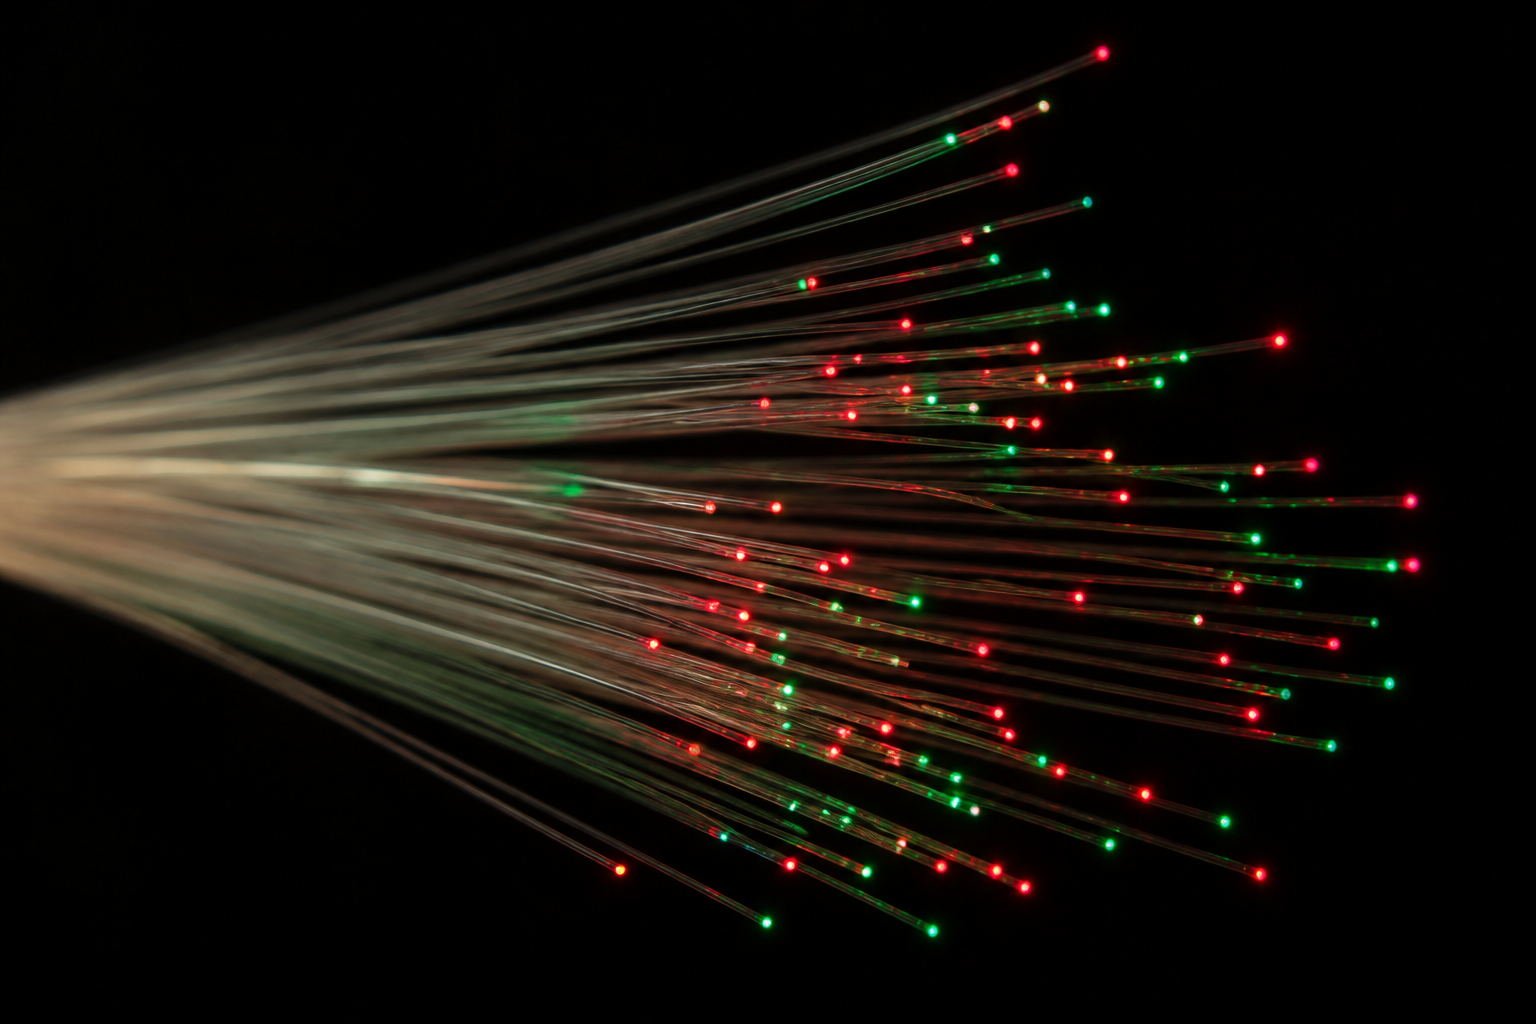
\includegraphics[width=0.58\linewidth]{images/book4/ai/b4-16-optical-fibres-glow.png}

{\small \omterm{prop:b2:guided-waves:fibre}{Serat optik} yang dinyalakan dari ujung jauhnya: cahaya yang terperangkap \omterm{thm:b2:wave-interfaces:snell}{pemantulan dalam total} dalam inti yang lebih tipis daripada sehelai rambut, dan dipandu mengelilingi setiap tikungan yang landai.}
\end{omfigure}

\section{Soal: Rongga oven dan serat optik}

\begin{problem}[{Soal akhir pekan --- dua sistem gelombang terpandu dalam setiap
dapur dan setiap kota: oven yang memasak dengan gelombang berdiri dan
serat yang mengemban internet}]
\label{pb:b2:guided-waves:1}

\medskip
\noindent\textbf{Bagian I --- Dari magnetron ke rongganya.}
Sebuah magnetron menyuapi \qty{800}{W} pada \qty{2.45}{GHz} ke dalam \omterm{prop:b2:guided-waves:rectangular}{pandu gelombang
bersegi empat} ($a = \qty{8.6}{cm}$, $b = \qty{4.3}{cm}$) yang membuka ke rongga
ovennya ($30 \times 30 \times 20$ cm$^3$); dindingnya baja, $\gamma = \qty{1e6}{S/m}$.
\begin{enumerate}
  \item Frekuensi ambang \omterm{prop:b2:guided-waves:rectangular}{ragam TE}$_{10}$, TE$_{20}$, TE$_{01}$ pandunya;
        periksalah bahwa hanya TE$_{10}$ yang merambat pada \qty{2.45}{GHz}.
  \item Panjang gelombang pandunya, \omterm{def:b2:dispersion-wave-packets:relation}{kecepatan fase} dan grupnya pada \qty{2.45}{GHz}.
  \item Amplitudo medan $E_0$ dalam pandunya bagi \qty{800}{W} (rumus daya
        TE$_{10}$); bandingkanlah dengan medan dadal udara.
  \item Amplitudo \omterm{prop:b2:maxwell-equations:boundary}{arus permukaan} pada dinding lebarnya (berorde
        $E_0/\mu_0c$); \omterm{def:b2:dispersion-wave-packets:complex}{kedalaman kulit} dan hambatan permukaan bajanya;
        rugi tiap meter pandunya.
  \item Ragam rongganya: daftarkanlah yang berfrekuensi dalam $3\%$
        dari \qty{2.45}{GHz} (cobalah $(m, n, p)$ sampai $4$); berapa banyak?
  \item Jarak antara bintik panas satu ragam semacam itu sepanjang tiap
        sumbunya; mengapa piringnya berputar, dan apa itu ``pengaduk ragam''?
  \item Faktor kualitas rongganya ketika terbebani makanan sekitar
        $200$: tentukanlah lebar pita tanggapannya; mengapa ketaksesuaian antara
        frekuensi magnetronnya dan ragamnya tak banyak berarti.
  \item Rongga kosongnya mempunyai $Q \approx 3000$: tentukanlah energi tersimpannya pada masukan
        \qty{800}{W}, rapat energi reratanya, amplitudo medannya; bandingkanlah dengan
        pertanyaan 3 dan dengan dadalnya. Apa yang melindungi magnetronnya
        ketika ovennya berjalan kosong?
  \item Waktu bagi energinya untuk menempuh \qty{20}{cm} pandu dari
        magnetronnya ke rongganya.
  \item Magnetronnya disuapi catu daya yang disearahkan setengah gelombang lalu memancar
        hanya selama separuh tiap daur jala-jalanya: tentukanlah daya puncaknya selama
        semburannya bagi rerata \qty{800}{W}; apa yang dilakukan rongganya
        di antara semburannya (pakailah $Q \approx 200$)?
\end{enumerate}

\medskip
\noindent\textbf{Bagian II --- Pintu dan ambangnya.}
\begin{enumerate}[resume]
  \item Jala pintunya mempunyai lubang \qty{1.5}{mm} pada lembar \qty{1}{mm}: tentukanlah panjang
        peluruhan dalam sebuah lubang dan \omterm{def:b2:dispersion-wave-packets:complex}{pelemahannya} dalam dB menyeberangi lembarnya.
  \item Tepi pintunya disekat sebuah ``cekikan'' seperempat gelombang: sebuah alur
        sedalam $\lambda/4$ mengelilingi kusen pintunya, yang menyajikan rangkaian
        terbuka pada celahnya (ingatlah \cref{ch:b2:wave-interfaces}): berapa dalam
        alurnya pada \qty{2.45}{GHz}.
  \item Kebocoran yang sah adalah \qty{5}{mW/cm^2} pada \qty{5}{cm}: itu setara dengan berapa bagian
        dari \qty{800}{W} yang menembus pintu \qty{100}{cm^2}?
  \item Sebuah cerobong \qty{30}{cm} berdiameter \qty{4}{cm} melubangi rongganya: adakah ia
        di bawah ambang pada \qty{2.45}{GHz}? Tentukanlah \omterm{def:b2:dispersion-wave-packets:complex}{pelemahannya} sepanjang panjangnya.
  \item Mengapa jalanya harus terhubung secara listrik ke kusen pintunya di
        seluruh kelilingnya (celah pada hubungannya akan berperilaku seperti apa)?
\end{enumerate}

\medskip
\noindent\textbf{Bagian III --- Seratnya.}
Sebuah serat indeks tangga: inti $n_1 = 1.465$, selongsong $n_2 = 1.460$, diameter
intinya \qty{50}{\micro m} (beragam banyak) atau \qty{9}{\micro m} (ragam tunggal);
$\lambda = \qty{1.55}{\micro m}$; \omterm{def:b2:dispersion-wave-packets:complex}{pelemahannya} \qty{0.2}{dB/km}.
\begin{enumerate}[resume]
  \item \omterm{prop:b2:guided-waves:fibre}{Apertur numerik} dan sudut penerimaannya; mudahkah mengopel
        cahaya ke dalamnya?
  \item Sebaran ragamnya tiap kilometer bagi serat beragam banyaknya; laju bit
        maksimum sepanjang \qty{10}{km} (satu bit tiap waktu sebarannya).
  \item Jumlah ragam serat beragam banyaknya (terimalah $N \approx
        \tfrac12(\pi d\,\mathrm{NA}/\lambda)^2$); dan yang ragam tunggal ($d =
        \qty{9}{\micro m}$: tunjukkanlah bahwa rumus yang sama memberi sekitar $1$).
  \item Dalam serat ragam tunggalnya penyebaran yang tersisa bersifat kromatik:
        dengan $\omega'' \approx \qty{-0.2}{m^2/s}$ (\cref{ch:b2:dispersion-wave-packets})
        dan pulsa \qty{50}{ps}, tentukanlah jarak yang sepanjangnya sebuah pulsa berlipat dua;
        laju bitnya sepanjang \qty{100}{km}.
  \item \omterm{def:b2:dispersion-wave-packets:complex}{Pelemahannya} sepanjang \qty{100}{km} dalam dB dan sebagai nisbah daya; masukan
        \qty{1}{mW}: tentukanlah daya keluarannya; dengan penguat tiap \qty{80}{km}, berapa
        banyak bagi sambungan lintas Atlantik \qty{6000}{km}?
  \item Frekuensi dan energi foton pada \qty{1.55}{\micro m}; foton tiap
        sekon dalam \qty{1}{mW}, dan tiap bit pada \qty{10}{Gbit/s}, pada masukannya
        dan sesudah \qty{100}{km}.
  \item Mengapa \qty{1.55}{\micro m} (pikirkanlah kedua mekanisme rugi
        silika: hamburan Rayleigh, yang turun sebagai $1/\lambda^4$, dan serapan
        inframerah yang naik di luar \qty{1.6}{\micro m})?
  \item Pemantulan Fresnel pada ujung serat yang dibelah dan menghadap udara: tentukanlah ruginya dalam
        dB; mengapa penyambungnya memakai gel penyesuai indeks atau sentuhan fisik
        yang dipoles.
  \item Mengapa sebuah serat tidak memancar pada tikungan yang landai, dan mengapa
        ia kehilangan cahaya pada tikungan yang tajam (pikirkanlah sudut sinarnya
        pada batas intinya)?
  \item Bandingkanlah kedua pandu soal ini: apa yang mengurung
        gelombangnya, apa yang membatasi lebar pitanya, apa ruginya.
\end{enumerate}
\end{problem}
